\documentclass[12pt]{report}
\usepackage[utf8]{inputenc}
\usepackage{graphicx}  % For including figures
\usepackage{amsmath}   % For math symbols
\usepackage{amssymb}   % For math symbols
\usepackage{hyperref}  % For clickable links
\usepackage{geometry}  % For setting margins
\usepackage{setspace}  % For setting line spacing
\usepackage{fancyhdr}  % For customizing headers
\usepackage{cite}      % For bibliography
\usepackage{lipsum}    % For placeholder text
\usepackage{titlesec}  % For section formatting
\usepackage{booktabs}  % For table lines
\usepackage{tikz}      % For drawing graphs
\usepackage{caption}   % For captions
\usepackage{float}     % For placing figures
\usepackage{subcaption} % For subfigures

\geometry{letterpaper, margin=1in}
\setstretch{1.5}  % 1.5 line spacing

\begin{document}

\chapter{Notation}

\begin{table}[ht]
    \centering
    \begin{tabular}{ll}
        \toprule
        \textbf{Symbol} & \textbf{Description} \\
        \midrule
        $G(V, E)$       & Graph with $V$ vertices and $E$ edges. \\
        $n = |V|$       & Number of vertices in graph $G$. \\
        $m = |E|$       & Number of edges in graph $G$. \\
        $A$             & The adjacency matrix for the graph $G$. \\
        $\Delta_i$      & Number of triangles node $i$ participates in. \\
        $d_i$           & Degree of node $i$. \\
        \bottomrule
    \end{tabular}
    \caption{List of notation used.}
    \label{tab:notation}
\end{table}

\newpage

\chapter{Literature Review}

\section{Outline DELETE LATER}
\begin{itemize}
    \item Why do we care about triangles? (Motivation)
    \item If we don't care about runtime, how do we calculate them? (Exact algorithms)
    \item Look, it's slow.
    \item Methods for fast triangle counting:
    \begin{itemize}
        \item Talk about different methods:
        \begin{itemize}
            \item Split into subsections:
            \begin{itemize}
                \item Linear algebraic methods (e.g. Eigentriangle, Hutchinson's estimator paper by Avron)
                \item Sampling methods
            \end{itemize}
        \end{itemize}
    \end{itemize}
    \item Our techniques that aren't specific to triangles:
    \begin{itemize}
        \item Importance sampling
        \item Variance reduction
        \item Learning-augmented algorithms
        \begin{itemize}
            \item If I have predictions about my output, how can I use them to augment my algorithms?
        \end{itemize}
        \item Talk about these techniques and where they've been used
    \end{itemize}
\end{itemize}

\section{Introduction}

Counting triangles is a fundamental problem in graph theory with widespread applications in social networks, bioinformatics, and more.
These triangles, formed by three mutually connected nodes, can, in social network graphs, represent closed friendships, indicating a high level of local connectivity, which can give great insight into the network as a whole.
However, for large graphs, especially sparse ones, where the number of edges is much smaller compared to the number of possible edges, efficiently counting these triangles poses significant computational challenges.

\section{Methods for Triangle Counting}

Triangle counting can be approached in a variety of ways, each with its advantages and drawbacks. 
One of the simplest methods is the brute force technique, where all distinct sets of three vertices ${u, v, w}$ are enumerated and checked for the existence of a triangle. This involves examining every possible combination of vertices in the graph and testing whether all three edges $(u, v)$, $(v, w)$, and $(w, u)$ exist. 

Assuming optimal conditions with edges stored in a hash table, where edge retrieval takes $O(1)$ time, the time complexity of this brute force approach is $\Theta(n^3)$. 
This cubic complexity arises because the number of combinations of three vertices grows cubically with the total number of vertices \cite{al_hasan_triangle_2018}. 

While this method is straightforward, it is inefficient for large graphs due to its high computational cost.
In smaller graphs, this runtime may be acceptable.
However, when scaling up to larger graphs—such as those representing extensive social networks, a $\Theta(n^3)$ runtime quickly becomes impractical.

Thus, researchers have turned to alternative triangle counting and estimation methods.

\subsection{Linear Algebraic Methods}

Graphs can be conveniently represented using adjacency matrices, which in social network analysis are typically referred to as \emph{sociomatrices} \cite{beum_method_1950}. 
In these matrices, each row and column represents a node, while edges between nodes are represented as 1s in the corresponding matrix entry.

\begin{figure}[H]
    \centering
    % Create a minipage for the graph
    \begin{minipage}{0.45\textwidth}
        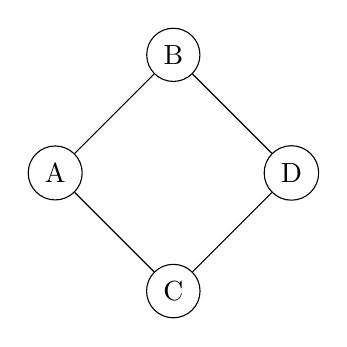
\begin{tikzpicture}[scale=1.5]
            % Define vertices
            \node[circle, draw] (A) at (0, 0) {A};
            \node[circle, draw] (B) at (1, 1) {B};
            \node[circle, draw] (C) at (1, -1) {C};
            \node[circle, draw] (D) at (2, 0) {D};

            % Draw edges
            \draw (A) -- (B);
            \draw (A) -- (C);
            \draw (B) -- (D);
            \draw (C) -- (D);
        \end{tikzpicture}
        \caption{Graph representation of vertices A, B, C, and D.}
    \end{minipage}%
    \hfill
    % Create a minipage for the adjacency matrix
    \begin{minipage}{0.45\textwidth}
        \[
        A =
        \begin{bmatrix}
        0 & 1 & 1 & 0 \\
        1 & 0 & 0 & 1 \\
        1 & 0 & 0 & 1 \\
        0 & 1 & 1 & 0 \\
        \end{bmatrix}
        \]
        \caption{Adjacency matrix corresponding to the graph.}
    \end{minipage}
\end{figure}

By using these adjacency matrices and leveraging linear algebra techniques, we can calculate triangle counts more efficiently. 
The trace of the matrix offers a simple and effective approach. Specifically, we can use the formula:

\[
\Delta = \frac{1}{6} \mathrm{trace}(A^3)
\]

This formula is derived from the fact that the diagonal elements of \(A^3\) count the number of triangles that each vertex participates in, effectively summing these counts across all vertices. 

To compute $A^3$, you first need to calculate $A^2$ (which takes $O(n^3)$ for an $n \times n$ matrix) and then multiply $A^2$ by $A$ (also $O(n^3)$).
Thus, the total complexity for computing $A^3$ is $O(n^3)$.
After computing $A^3$, calculating the trace takes $O(n)$, as you need to iterate over the $n$ diagonal elements.
Thus, the overall runtime complexity for the operation is $O(n^3)$.

\subsubsection{Strassen's Algorithm}

This previous approach assumes that matrix multiplication is performed using the standard algorithm.
However, more sophisticated techniques, such as Strassen's algorithm \cite{strassen_gaussian_1969}, can reduce matrix multiplication time.
Strassen's algorithm divides each matrix into smaller submatrices and performs a series of additions and multiplications that require only seven multiplications of these smaller matrices instead of eight, which is typical in standard matrix multiplication.

For large, square matrices, such as sociomatrices, Strassen's algorithm reduces the complexity of multiplying two $n \times n$ matrices to approximately $O(n^{\log_2 7})$, which is about $O(n^{2.81})$.
Computing $A^2$ using Strassen's algorithm will take $O(n^{\log_2 7})$.
Then, multiplying $A^2$ by $A$ again takes $O(n^{2.81})$.
Therefore, the total complexity for computing $A^3$ with Strassen's algorithm is $O(n^{\log_2 7}) + O(n^{\log_2 7}) = O(n^{\log_2 7})$, or roughly $O(n^{2.81})$.

\subsubsection{EigenTriangle Algorithm}

Another significant approach in triangle counting is the use of spectral methods.
One such method is the EigenTriangle algorithm \cite{tsourakakis_fast_2008}, which estimates the triangle count $\Delta$ by considering the spectral decomposition of the adjacency matrix $A$.

The EigenTriangle algorithm is based on the observation that the number of triangles in a graph is closely related to the spectrum of its adjacency matrix.
In particular, the adjacency matrix $A$ is decomposed as:

\[
A = U \Lambda U^T
\]

where $U$ is a matrix whose columns are the eigenvectors of $A$, and $\Lambda$ is a diagonal matrix containing the corresponding eigenvalues.
The cube of the adjacency matrix $A^3$ can be approximated by considering the largest eigenvalues and their corresponding eigenvectors, significantly reducing the computational complexity when compared to the direct calculation of $A^3$.

Once the decomposition is performed, the number of triangles can be estimated using:

\[
\Delta \approx \frac{1}{6} \sum_{i=1}^{k} \lambda_i^3
\]

where $\lambda_i$ are the $k$ top eigenvalues of the adjacency matrix.
The runtime of EigenTriangle is dominated by the cost of computing the top $k$ eigenvalues and eigenvectors of $A$, which can be done in $O(k m)$, where $m$ is the number of edges and $k$ is typically much smaller than the number of nodes $n$.
This is a substantial improvement over the complexity of direct methods like $\mathrm{trace}(A^3)$.

\subsection{Randomized Algorithms}

To address this, we turn toward randomized algorithms. These algorithms rely on probabilistic techniques to sample subsets of the graph's nodes, estimating the global triangle count based on local observations.
By doing this, these algorithms significantly reduce the runtime compared to exact methods, particularly in sparse graphs where only a fraction of potential edges exist.

Additionally, randomized algorithms often provide tunable accuracy, allowing for a trade-off between precision and performance, making them ideal for processing large-scale networks.

\newpage
\bibliographystyle{plain}
\bibliography{thesis_bib}

\end{document}
